\subsection{Mallob Integration}
In this section we will give an overview over how we integrated CrowdHTN with Mallob. More information about how to do this for general problems can be found in the Mallob GitHub repository \footnote{https://github.com/domschrei/mallob}. There are three steps we need to perform:
\begin{itemize}
	\item Implement a way to read and encode a TOHTN instance
	\item Implement the Mallob job interface seen at \ref{algo - mallob interface}
	\item Implement a way to encode a result for writing to file
\end{itemize}
As we discussed in section \todo{ref the proper sub thingy once it exists} on how we designed malleable CrowdHTN, we choose to communicate an instance by simply transferring the contents of the instance file, making the first step easy. The third step, encoding a result for writing, is similarly easy as CrowdHTN already contained a mechanism to write a plan to the terminal. Most of the work was done in the second step which we will now discuss in more detail. As a general principle, CrowdHTN was kept as a separate library which is linked into Mallob. The implementation of the TOHTN job within Mallob is a wrapper around this library. This allowed for a clearer separation of concerns where our job implementation does not need to know anything about the specifics of TOHTN planning while CrowdHTN is agnostic of implementation details its environment, e.g. how messages are transmitted.\\
Both CrowdHTN and Mallob are implemented using the C++ programming language.
\begin{algorithm}
	\caption{The Mallob job interface}
	\label{algo - mallob interface}
	void appl\_start()\;
	void appl\_suspend()\;
	void appl\_resume()\;
	void appl\_terminate()\;
	void appl\_solved()\;
	JobResult appl\_getResult()\;
	void appl\_communicate()\;
	void appl\_communicate(source, mpi\_tag, message)\;
	void appl\_memoryPanic()\;
\end{algorithm}
\begin{comment}
- how we integrated CrowdHTN with Mallob
- the interface code can be found online in the Mallob repository 

- three things:
- how to read a problem instance, in our case a TOHTN instance
- how to create a new job
- how to properly write the result to file in a meaningful way

- this is done by implementing a job interface in Mallob

- and additionally a function to read an instance
- give a short overview of the interface
\end{comment}

\paragraph{Implementing the Job Interface}
In this paragraph we explain how we implemented the Mallob job interface for CrowdHTN while upholding the guarantees demanded by Mallob. For ease of reading we will leave out the \textit{appl} prefix shared by all functions. \\
The Mallob job interface can be split into four parts. First, a worker in Mallob is implemented as a state machine with \textit{start}, \textit{suspend}, \textit{resume} and \textit{terminate} responsible for the transitions. The corresponding state diagram can be seen in figure \ref{figure: mallob state diagram}. Second, the two \textit{communicate} calls allow for communication. For general communication we note that Mallob requires all communication calls to take place in the main thread, i.e. we may not send any messages in any threads we started to perform internal work. For ease of separation we further restrict ourselves to only send messages in the \textit{communicate} calls. Third, we have the functions \textit{solved} and \textit{getResult} for general bookkeeping regarding solutions. Last, we have \textit{memoryPanic} which signals the job that memory usage is critically high. We discuss it's use in the next paragraph. \\
As \cite{schreiber2021scalable} writes, Mallob aims to achieve millisecond latencies. To enable this goal, we may not block the main thread any longer than a few milliseconds at most and must keep work performed directly in any of the job interface functions to a minimum. We achieve this by delegating all planning and handling of the CrowdHTN library to a separate work thread which is initialized in the \textit{start} function. This work thread is the only thread ever directly interacting with CrowdHTN. Due to this, we avoid locking on CrowdHTN which also allows us to keep working at all times. State transitions are communicated to the work thread via a number of atomic variables, \textit{suspend} and \textit{resume} additionally use a condition variable to suspend and wake up the work thread. \\
To be able to keep communication to the \textit{communicate} functions, the job and the work thread exchange messages via separate buffers. While these buffers do necessitate locking, we restrict the critical section to be at most a copy of a few bytes. \\
The last problem is the \textit{start} call during which we need to parse our TOHTN instance, setup the CrowdHTN data structures and start our worker thread. Here both the parsing of the instance and, within CrowdHTN, computing the heuristic values may take longer than Mallob allows. For this reason, we have decided to place the initialization itself into a separate thread and return fast.
\begin{comment}
\todo{job is a state machine, the functions guide us through this state diagram}
- a job is internally implemented as a state machine
- the state diagram is found at \ref{figure: mallob state diagram}
\begin{figure}
\caption{State transition diagram of a Mallob job}
\label{figure: mallob state diagram}
\centering
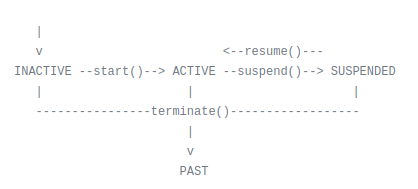
\includegraphics{images/prelim/mallob_state_diagram}
\end{figure}

- from \cite{schreiber2021scalable} we know that Mallob aims to deliver latencies in the millisecond range
- messages may only ever be sent from the main thread

- initialization in \textit{start} is performed in a separate thread (parsing the instance, constructing the data structures for CrowdHTN)

- CrowdHTN is run in a separate work thread
- only this work thread ever directly accesses CrowdHTN
- never locking on CrowdHTN allows us to keep performance high
- communication is done via \textit{std::atomic} provided by the C++ STL
- \textit{suspend}, \textit{terminate}, requests for data
- locks are then only used for the buffers in which messages are stored
- critical section is minimal, normally only used for a few small copies
- operating system facilities are used where they apply, e.g. condition variables to implement \textit{appl\_suspend} and \textit{appl\_resume}
\end{comment}

\paragraph{Added Fault Tolerance}
As a scheduler, within a single execution Mallob may work on any number of jobs making it necessary that jobs do not crash. This imposes additional challenges for TOHTN planning, as we have seen in section \ref{prelim: tohtn complexity} that TOHTN planning is EXPSPACE hard, meaning we may often run out of memory and will be subsequently shut down by the operating system. Luckily, the Mallob job interface we see in algorithm \ref{algo - mallob interface} does provide a function for this case. Mallob does periodically check available memory and if it threatens to run out triggers the \textit{appl\_memoryPanic()} function. In our case we have implemented it as clearing out both our local fringe of search nodes and the loop detection information, resetting the local search. Afterwards, an affected PE will simply resume the work stealing and message other PEs to re-join the work at reduced memory footprint. While this does means we loose parts of the search space, the alternative would be to immediately return without a plan. Additionally, with the restarting mechanism we introduced in section \ref{ld - completeness} CrowdHTN retains completeness even in this case.

\paragraph{TODO: Messages by dead workers}
\todo{fill this}

\subsection{Efficiently Handling Version Increases}
In our malleable CrowdHTN implementation, version increases show up in a number of ways. They are necessitated by the global loop detection introduced in section \ref{improv: loop detection} and further allow our DFS based planner to achieve completeness as explained in section \ref{improv: completeness}. Due to the distributed fashion in which CrowdHTN operates, version updates are not perfectly synchronized and workers may be at different versions. We will now outline how correctness is ensured and how versions are propagated efficiently. \\
While versions between workers may differ, we must ensure that especially work packages of different versions are not mixed as to not duplicate parts of the search space. This is ensured by attaching the worker version to any outgoing messages. Upon receiving a message, a worker first decodes the version. If this incoming version is higher than the internal version, the internal version is updated, the local fringe and loop detection cleared and the message is then handled according to this new internal state. If the incoming version is lower, depending on message type it is ignored (e.g. for work packages) or responded to normally (e.g. for work requests). Including the version with all messages has an additional use when integrating new PEs. As they start out empty and without a way to know the current version, they will immediately send out a work request to a random other worker and receive both the current version and potentially their first work package, requiring no special handling. \\
Including the version in each message is already sufficient to propagate the version to all workers. However, if we disable global loop detection there are no regular broadcasts from the root to the other PEs. Additionally, the work represented by a search node and it's children may be arbitrarily large. While this reduces the amount of messages sent and is one of the strengths of work stealing in parallel TOHTN planning, it also results in a potentially slow propagation of version increases, having many workers perform outdated work. To counter this problem, whenever a version increase happens at the root PE we start a version broadcast along the binary tree structure of PEs. This ensures that all PEs adopt the new version in a timely manner.

\subsection{Global Loop Detection}
In section \ref{ld - global} we introduced a distributed loop detection mechanism based on regularly shared bloom filters. This leaves us with two problems, first performing the associated allreduction while the PEs assigned to the job may change at any time and secondly performing the restarts which are required if the bloom filter fills up. \\
In both cases we will make use of the specific way in which Mallob organizes the PEs assigned to a job which we have already explained in section \ref{prelim: mallob}. The two properties we rely on are the fact that PEs are internally structured as a binary tree with parent and child information available to us and the fact that the root PE will remain assigned to a job during the job's full duration.

\paragraph{Performing the Reduction}
The all-reduction of our loop detection data is initiated by the root PE and performed in three phases. 
\begin{itemize}
	\item Initiating the reduction
	\item Aggregating information upwards
	\item Broadcasting the aggregated information
\end{itemize}
The root PE is responsible for initializing the all-reduction. It does so by starting a broadcast, sending an initialization message to all it's children. Upon receiving a reduction initialization message, a PE both forwards the message to its own children and prepares the local loop detection data. At the leaves, this data can immediately be sent upwards whereas inner nodes wait until they have received data from all children before performing their local aggregation and forwarding the result upwards. As we combine the bloom filters via a bitwise or operation the message size stays constant throughout. Once the root has received data from all children it once again starts a broadcast, this time containing the aggregated data. \\
Starting the reduction with the initial broadcast allows us to easily coordinate all PEs even as PEs may assigned to our job may change at any moment. Similarly, we have to deal with PEs leaving at any time. This may be communicated to us either through getting our initial broadcast returned as no receiver is available or by having the \textit{appl\_suspend()} function called on us by Mallob. In both cases we simply substitute the message of the missing PE with a response that simulates empty data. We note that, due to changing PEs, the sets of PEs which broadcast their data and which receive the aggregated data may be different. Furthermore, neither of these two sets needs to correspond to the actual tree of PEs assigned to the job at any given time, as this set may change during the broadcast.

\begin{comment}
- init: allows for a centralized start

- multiple phases:
- 
- root induces a new sharing operation, broadcasting this information

- receiving PEs initiate their local operation, get local data, forward broadcast
- from the leaves we propagate the information upwards
- if the initiation broadcast is returned or a worker is suspended after receiving it, it's parent pretends that a message containing no data was sent
- this whole operation takes logarithmic time in the number of PEs
- if we enforce 'response exists' from bottom to top we will always conclude the operation even when PEs change
\end{comment}

\paragraph{Loop Detection Induced Restarts}
In section \ref{ld - global} we introduced a global loop detection mechanism based on regularly shared bloom filters. One of the problems this induces is that we need to induce restarts to increase the size of the bloom filter in order to avoid increasing false positive rates. The main problem here is that for different PEs the global bloom filter will fill up at different times. This is due to the fact that different PEs may be assigned to our job for different spans in time which may be further disjointed as PEs are suspended and subsequently reassigned to a job. However, to uphold our guarantees we want to restart all our PEs as soon as a single PE needs to do so.\\
To solve this, we rely on the fact that the root PE is guaranteed to remain assigned to a job during the job's full lifetime. Due to this, the root PE takes part in every single loop detection data exchange and it's global filter will contain at least as much data as any other PE's filter. This fact allows us to only ever check on the root PE whether the global bloom filter is full and institute a restart if needed. Doing so lets us avoid any problems that would stem from all PEs performing such checks, such as multiple PEs instituting restarts at the same time.
